\documentclass[a4paper]{scrreprt}

\usepackage[T1]{fontenc}
\usepackage[utf8]{inputenc}
\pdfoptionpdfminorversion 7
\usepackage{graphicx}
\usepackage{svg}
\usepackage{listings}
%\usepackage{showframe}
\usepackage{fullpage}
\usepackage[colorlinks=true]{hyperref}
\usepackage{tabu}
\usepackage{float}
\usepackage{afterpage}
\usepackage{pdflscape}
\usepackage{pdfpages}
\usepackage[abs]{overpic}
\usepackage{nth}

\lstdefinelanguage[ARM]{Assembly}     % add a "x64" dialect of Assemblers
   [x86masm]{Assembler} % based on the "x86masm" dialect
   % with these extra keywords:
   {
   morekeywords={ADDS, ANDS, B, LDR, MOV, ORRS},
    morekeywords=[2]{.align,.cpu,.thumb,.syntax,.word},%
    alsoletter={.,0,1,2,3,4,5,6,7,8,9},%
    alsodigit={?},%
    sensitive=false,%
    morestring=[b]",%
    morecomment=[s]{/*}{*/},%
    morecomment=[l]@,%
    morecomment=[l]//,%
   }[keywords,comments,strings]
\lstset{language=[ARM]Assembly}

\title{\vspace*{60mm}Introduction to Microcontrollers Notes}
\author{James Gowans}

\begin{document}
  \maketitle

  \vspace{\fill}
\section*{Licence}
This work is licensed under the Creative Commons Attribution-ShareAlike 3.0 Unported License. To view a copy of this license, visit http://creativecommons.org/licenses/by-sa/3.0/ or send a letter to Creative Commons, 444 Castro Street, Suite 900, Mountain View, California, 94041, USA.


\newpage
\tableofcontents
\newpage
%\section{A History of Processing}
In 1971 the dawn of a new era began. Intel had just announced that they had developed ``a programmable computer on a chip.'' The chip, known as the 4004 was the first general purpose microprocessor on one silicon chip, and contained around 2300 transistors. In order to produce this chip, the layout of the transistors was hand-drawn using coloured pencils at 500 times scale. The CPU had the ability to transfer 4 bits per clock cycle, had a 12-bit address space and an 8-bit instruction. In total, it has 16 instructions which it could execute. It was used in a calculator which had an optional square root function. The calculator run around 100K instructions per second, had 1 KB of ROM and 80 bytes of RAM. 

The next year, in 1972 Intel released the 8008, an 8-bit microprocessor. The 8008 had a 14 bit address space. The first use for the 8008 was a programmable scientific calculator. In 1973 the 8008 was used as the CPU for a French desktop computer. Some consider this to be the first desktop computer. The 8008 evolved into the 8080. 

While desktop computers do take a large share of the microprocessor market, many times more microprocessors go into microcontrollers for the purpose of embedded control applications. In 1996, 25 years after the advent of the first microprocessor, 70\% of all semiconductors are used for microcontroller-based circuits. 

A processor with IO an memory is a microcontroller. In 1995, 50\% of microcontrollers manufacturered were 4-bit. 

\chapter{System Overview}

\begin{figure}[t]
  \centering
  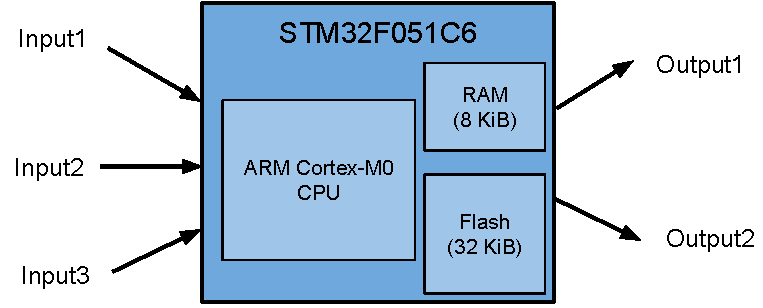
\includegraphics[width=\textwidth]{./week1/programmers_model_v0.pdf}
  \caption{The most simplified view of the internals of the STM32F051}
  \label{fig:prog_mod_v0}
\end{figure}

\section{What is a Microcontroller?}
The microcontroller can be understood by comparing it to something you are already very familiar with: the computer. Both a microcontroller and a computer can be modeled as a black box which takes in data and instructions, performs processing, and provides output.
In order to do this, a micro has some of the same internals as a computer, shown graphically in \autoref{fig:prog_mod_v0} and discussed now:
\begin{itemize}
  \item CPU: The section of the microcontroller which does the processing. It executes instructions which allows it to do arithmetic and logic operations, amongst other forms of operations.
  \item  Volatile memory (RAM:) This is general purpose memory. It can be used for storing whatever you want to store in it. Typically it stores variables which are created or changed during the course of execution of a program.
  \item Non-volatile memory (Flash): This non-volatile memory is used to store any date which must not be lost when the power to the micro is removed. Typically this would include the program code and any constants or initial values of data.
  \item Ports: Interfaces for data to move in and out of the micro. This allow it to communicate with the outside world. 
\end{itemize} 
These resources are typically orders of magnitude smaller or a micro than on a conventional computer. A micro makes up for this lack of resources with a small size, low power and low cost. A comparison of the characteristics can be seen in \autoref{table:specs_comp}.
A computer is typically defined as a multi-purpose, flexible unit able to do computation. A microcontroller on the other hand typically is hard-coded to do one specific job.\\

\begin{table}
\begin{tabu}{ >{\textbf}c | c  c  c  c  c  c }
  & \textbf{CPU} & \textbf{RAM} & \textbf{Non-volatile} & \textbf{Power} & \textbf{Size/Mass} & \textbf{Cost} \\
  \hline
  \textbf{Computer} & Dual, 3 GHz & 4 GiB & 500 GB & 100 W & Large & R 3000 \\
  \textbf{Micro} & 48 MHz & 8 KiB & 32 KiB & 50 mW & Small & R 15 \\
\end{tabu}
\caption{Comparison of specs of entry level computer to STM32F051C6.}
\label{table:specs_comp}
\end{table}

The terms \textit{microcontroller} and \textit{microprocessor} are different and should not be used interchangeably. A micro\textit{processor} is an IC which is able to perform computation, but requires external memory and peripherals to function. A micro\textit{controller} has the memory and peripherals built into it, allowing it to be fully independent. Furthermore, the interface in and out of a microprocessor is mainly just an address and data bus. In a microcontroller, these busses are internal to the device. The interfaces in and out of a microcontroller are configurable to be a wide variety of communication standards. This self-contained nature and ability to deal with a wide variert of signals allows a microcontroller to (as the name suggest) be embedded in a larger system and perform control and monitoring functions.\\

The micro we will be using is the STM32F051C6. It is manufactured by ST Microelectronics, but has an ARM Cortex-M0 CPU. ARM designed the CPU (specified how the transistors connect together). ST then takes this CPU design, adds it to their design for all of the other bits of the micro (flash, RAM, ports and much much more) and then produces the chip.

\subsection{Development board block diagram}
The development board consists of modules which connect to the microcontroller. Most of these modules are optional in that they are not required for the microcontroller to run. We will develop code later in the course to interface with some of these modules. Those which are not optional are the voltage regulator and the debugger.
Following is a brief discussion of the purpose of each of the dev board modules (peripherals).

\begin{figure}
  \centering
  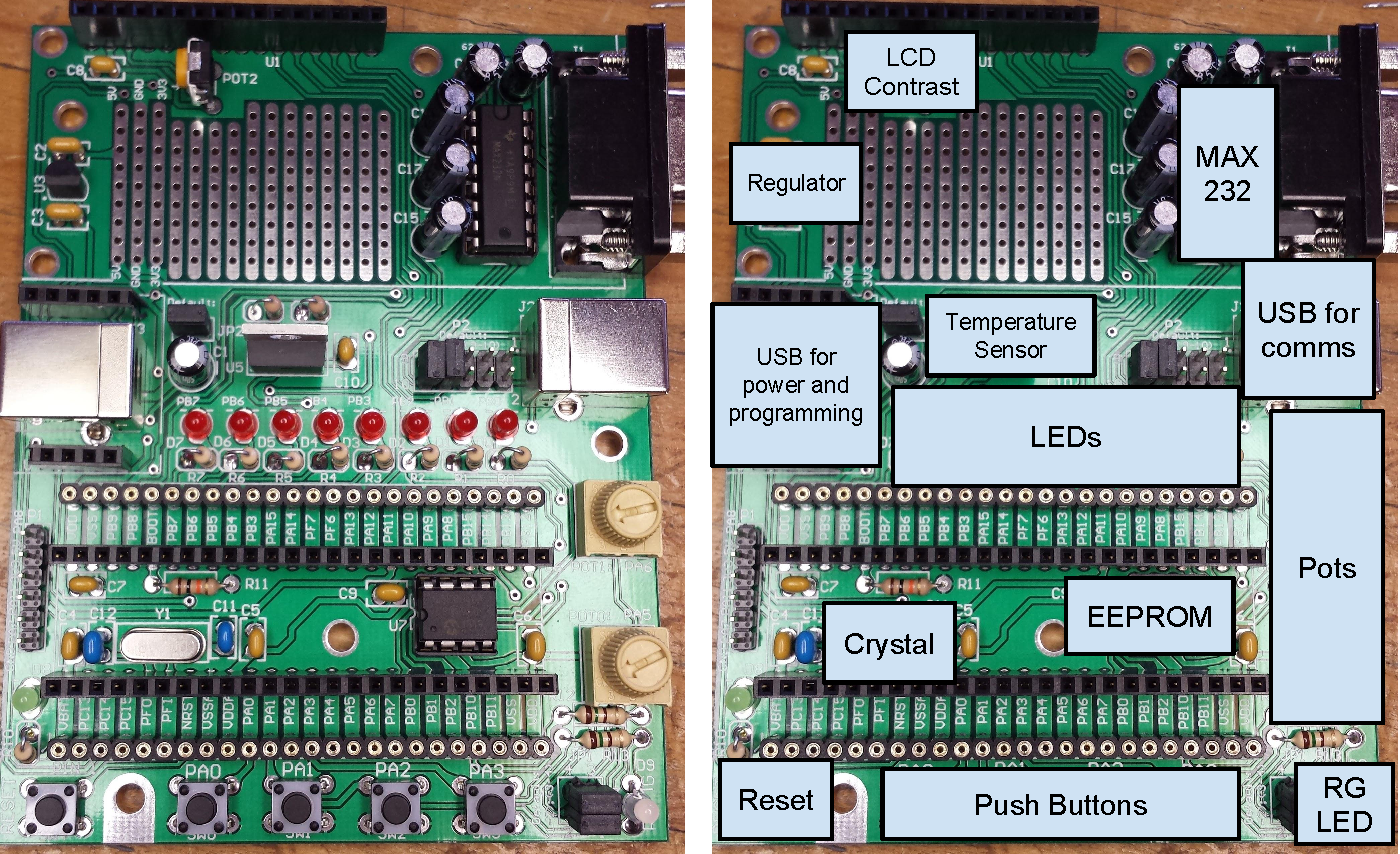
\includegraphics[width=\textwidth]{./week1/dev_board_unplugged.pdf}\\
  \vspace{3mm}
  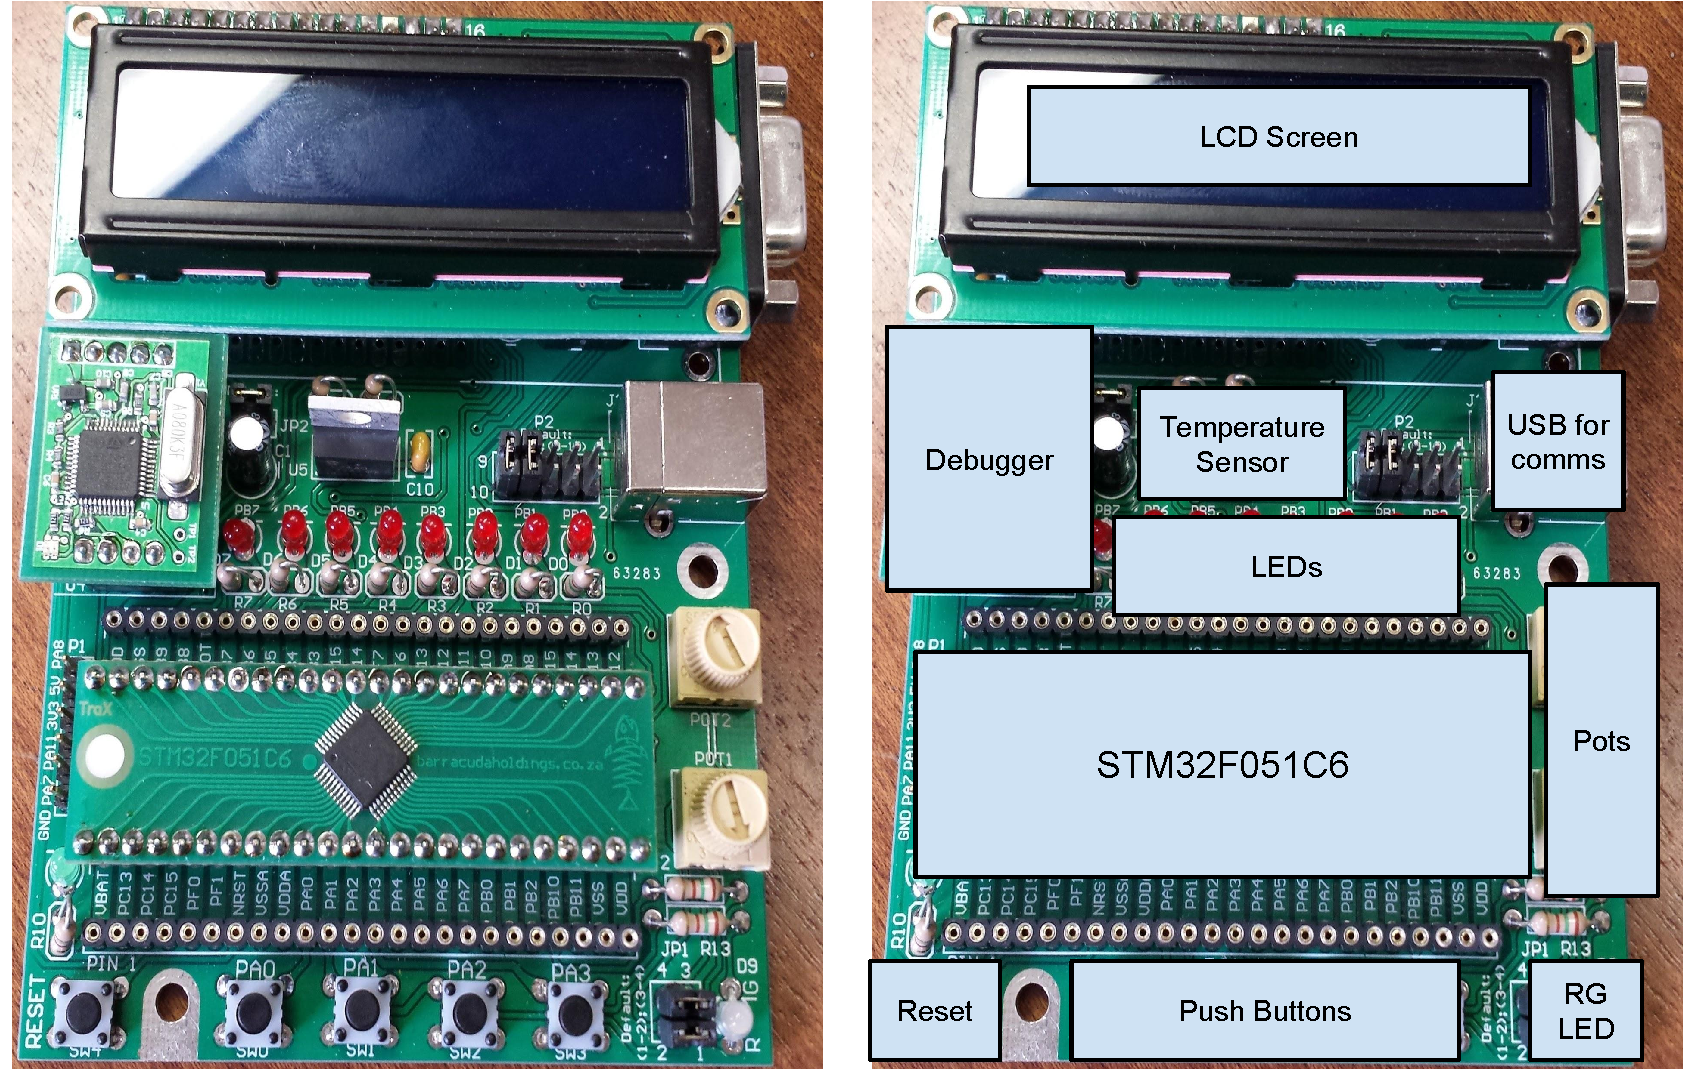
\includegraphics[width=\textwidth]{./week1/dev_board_plugged_in.pdf}
  \caption{Modules on the dev board as seen when top boards unplugged or plugged in.}
\end{figure}

\begin{itemize}
  \item STM32F051C6: This is the target microcontroller. It is connected to everything else on the board and it is where the code which we develop will execute. 
  \item Debugger: this is essentially another microcontroller running special code on it which allows it to be able to pass information between a computer and the target microcontroller. The interface to the computer is a USB connection, and the interface to the target is a protocol called Serial Wire Debug (SWD) which is similar to JTAG. The specific type of debugger which we have is a ST-Link.
  \item Regulator: A MCP1702-33/T0 chip. This converts the 5 V provided by the USB port into 3.3 V suitable for running most of the circuitry on the board. 
  \item LEDs: One byte of LEDs, active high connected to the lower byte of port B.
  \item Push buttons: Active low push buttons connected to the lower nibble of port A.
  \item Pots: 2 x 10K (or there abouts) potentiometers connected to PA5 and PA6.
  \item LCD Screen: A 16x2 screen connected to the micro in 4-bit mode. Used to display text.
  \item LCD contrast pot: The output of this potentiometer connects to the contrast pin of the LCD screen, hence allowing contrast adjustment.
  \item MAX232: This chips translates between TTL or CMOST logic level UART traffic and bi-polar higher voltage RS-232 traffic. Used for industrial communications links.
  \item USB for comms: The header allows intercepting of the UART traffic before it gets to the MAX232 and converting it to USB traffic through a small board which plugs into that header. When this facility is not being used, the jumpers on the header should be placed to allow the UART traffic to make its way to the MAX232.
  \item Temperature sensor: A TC74-A0 $I^2C$ temperature sensor.
  \item Crystal: 8 MHz quartz oscillator with 10 pF caps for removing high frequency harmonics. 
  \item EEPROM: A 25LC640A 64Kb Electronically Erasable and Programmable Read Only Memory (EEPROM) chip which communicates over SPI.
  \item RG LED: Common cathode Red/Green LED.
\end{itemize}


The full circuit schematic for the board follows. 
For now, we will forget about all of the other modules on the dev board and consider our system to be a computer talking to a debugger talking to a target micro, as shown in \autoref{fig:debugger_to_micro}. 
This is the most basic system which must be understood to allow us to load code onto the target microcontroller.

\begin{figure}[t]
  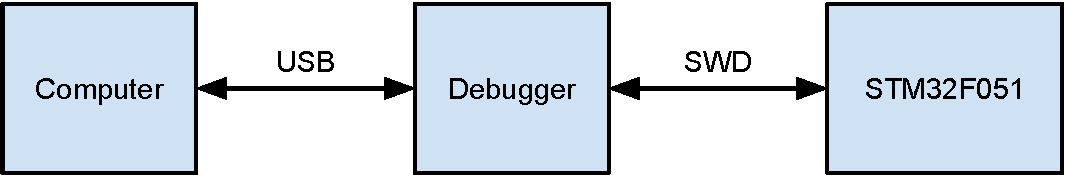
\includegraphics[width=\textwidth]{./week1/debugger_to_micro.pdf}
  \caption{Highly simpified diagram showing how micro and computer communicate}
  \label{fig:debugger_to_micro}
\end{figure}

\afterpage{
  \begin{landscape}
  %\begin{figure}
    \centering
    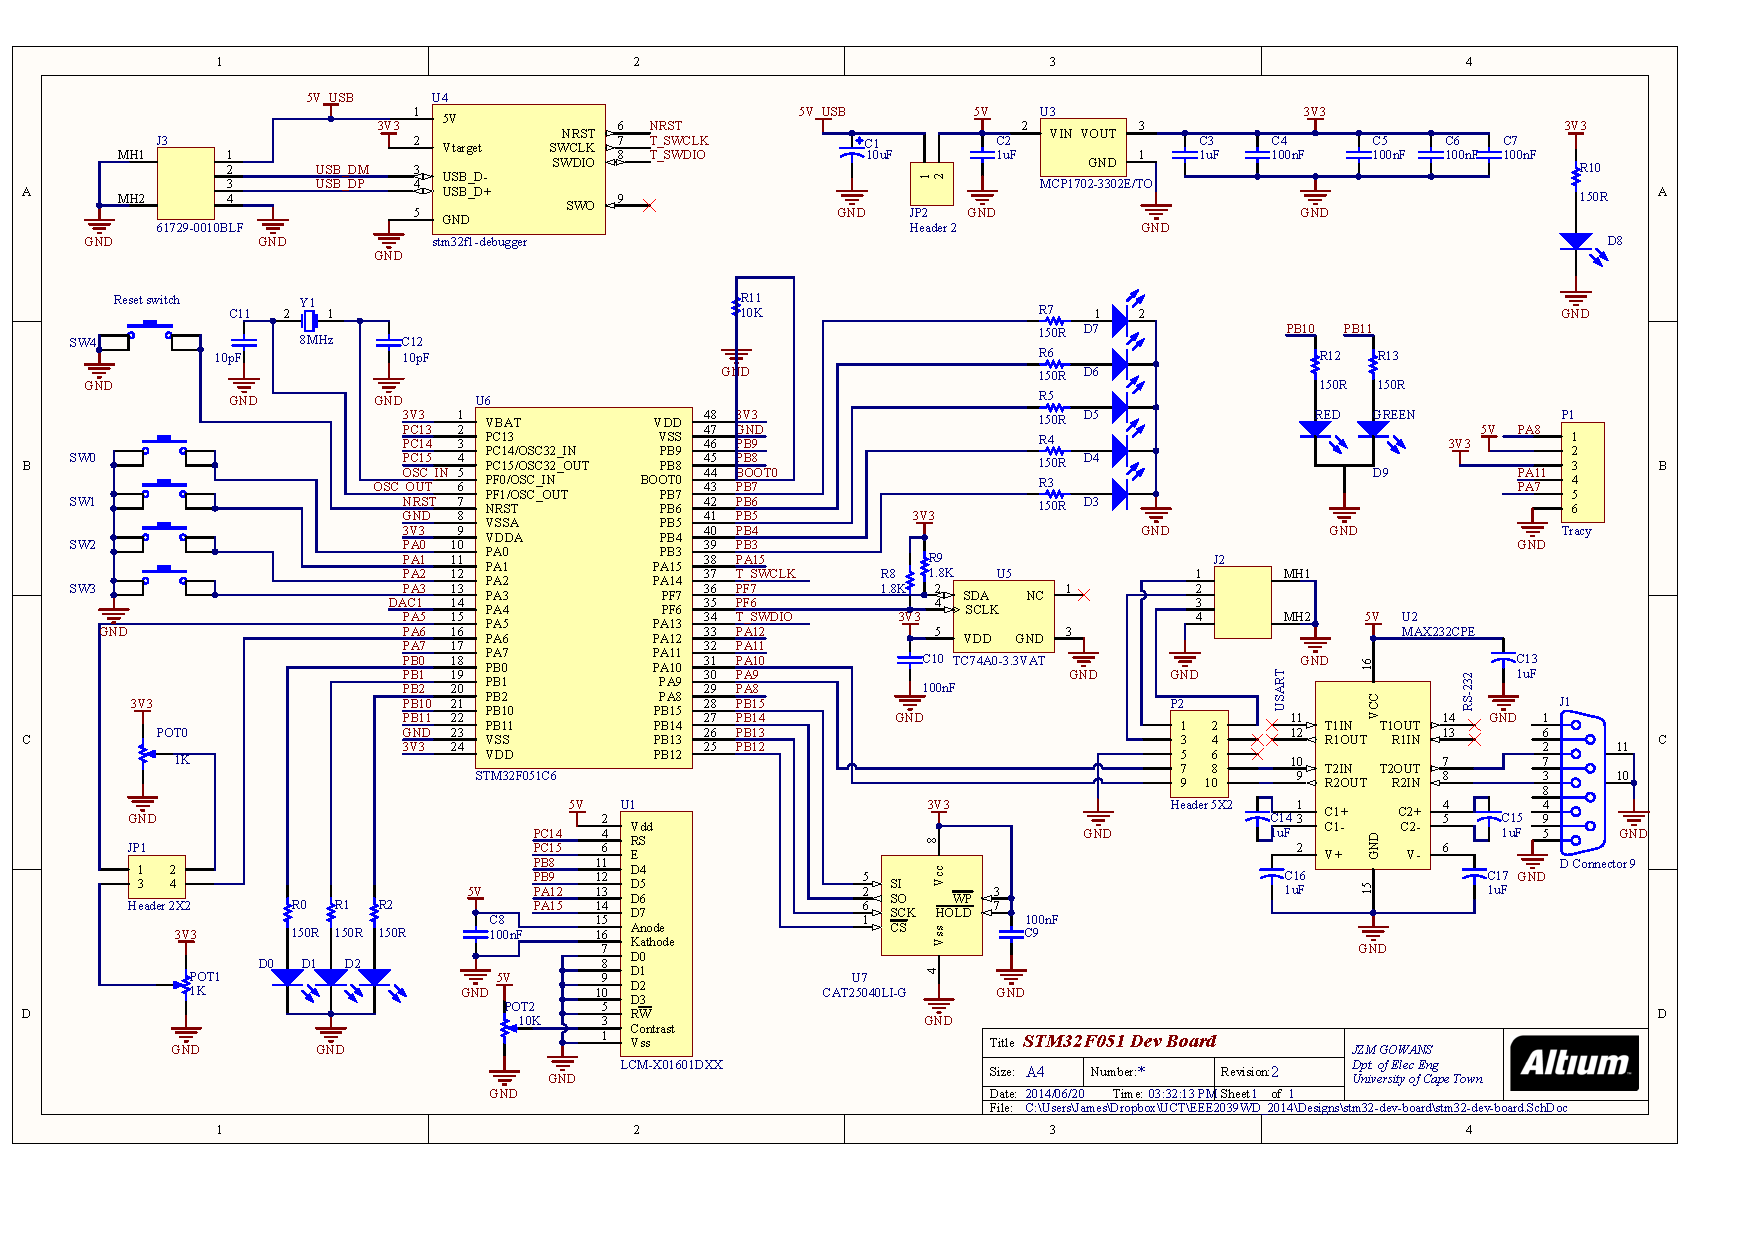
\includepdf[pages={1}, angle=90]{./week1/circuit_sch.pdf}
 % \end{figure}
 \end{landscape}
} 







%\subsection{A Short History of ARM}
%Acorn

%\chapter{Perihperals}
%Ports are typically controlled by a block of memory called perihperals. Unlike RAM which is general purpose, each register in the perihperals memory block has a specific, well defined purpose. Typically the purpose of these perihperal registes are for configuring the microcontroller to behave in a certain way or communicate with the outside world.
%These CPU registers are different to the peripheral registers mentioned earlier for the reasons that they are located inside the CPU rather than in the address space and also they are mostly general purpose: they can hold any data required in the execution of a program. 


\chapter{Memory Model}
We will now beging to expand on some of the block is \autoref{fig:prog_mod_v0}. Before starting to explore how the CPU works, it's useful to have an understanding of how memory is laid out. We will start looking at the flash and RAM blocks. Together with another block called perihperals (which we will explore later), these blocks make up memory. 
It's important to note that this memory is located \emph{outside} of the CPU, but still inside the microcontroller IC.

The memory of a device can be though of as a very long row of post boxes along a street. 
Each post box has an address, and each post box can have data put into it or taken out. The amount of data that each post box can hold is 8 bits, or one byte. Therefore, each memory address is said to address one byte. 
The address of each post box is 32 bits long, meaning that addresses range from 0 (0x00000000) to just over 4.3 billion (0xFFFFFFFF). In actual fact, the \emph{vast} majority of these addresses do not have a post box at them. These addresses are said to be unimplemented. 
Only very small sections of this address space are implemented and can actually be read from or written to.
Flash and RAM are contiguous blocks of memory, with a start address and an end address. A simplified memory map of the STM32F051 is shown in \autoref{fig:memory_map}. From this, we can see that if we want to use changeable variables in our programs, the variables should be located at addresses between 0x2000 0000 and 0x2000 1FFF. If we want to load code onto the micro which should not be lost when the device loses power, the code should be loaded into the non-volatile memory, flash, which has addresses between 0x0800 0000 and 0x0800 7FFF.
If we want the ability to modify data during the execution of our program, the data should be placed in the read/write section of memory, RAM. 

\begin{figure}
  \centering
  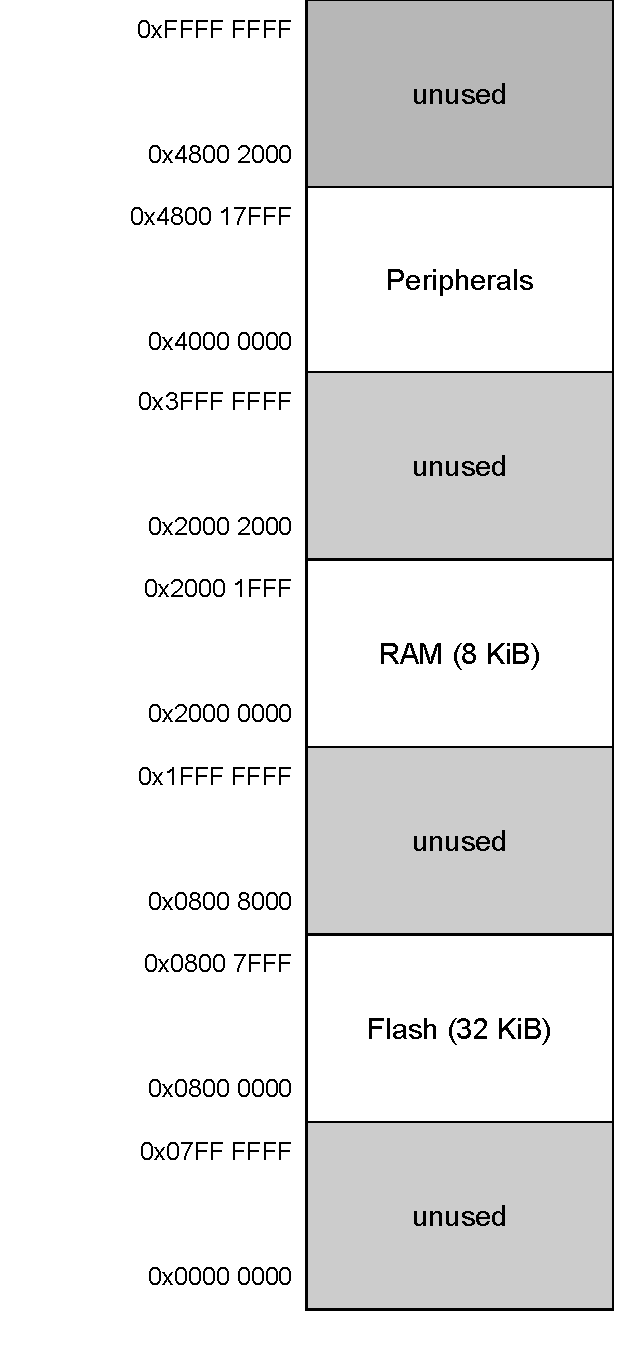
\includegraphics[width=0.6\textwidth]{./week1/memory_model_v0.pdf}
  \caption{Simplified STM32F051C6 memory map. Note how all addresses are 32 bits. The blocks are very much not to scale. Source: datasheet, Figure 9}
  \label{fig:memory_map}
\end{figure}

\section{Data Types and Endianness}
Very often we will need to work with clumps of data which are larger than 1 byte. ARM defines datatypes for a 32 bit CPU as follows:
\begin{itemize}
  \item byte: 8 bits
  \item halfword: 16 bits
  \item word: 32 bits
  \item doubleword: 64 bits
\end{itemize}
Each memory address only addresses one byte of memory, so how can something like a word (four bytes) be stored in memory? 
Obviously, the four bytes have to come after each other to form a four byte block, or word.
However, it is not obvious which order they should come in. For example, consider the case of wanting to store the word 0xAABBCCDD in address 0. The two possible ways of doing it are shown in \autoref{tab:endianness}. It doesn't really matter which one of these schemes is used - they each have their pros and cons and different processors use different methods. It is important to know which one our processor has chosen to use. Our processor uses little endian. A more abstract view of how data is stored in our processor is given in \autoref{fig:little_end_prog_man}
\newpage
\begin{table}
\centering
\begin{tabu}{cc}
    \multicolumn{2}{c}{\textbf{Little Endian}}\\
    \hline
    Address & Data \\
      \hline
      3 & 0xAA \\
      2 & 0xBB \\
      1 & 0xCC \\
      0 & 0xDD \\
\end{tabu}
\qquad
\begin{tabu}{cc}
    \multicolumn{2}{c}{\textbf{Big Endian}}\\
    \hline
    Address & Data \\
      \hline
      3 & 0xDD \\
      2 & 0xCC \\
      1 & 0xBB \\
      0 & 0xAA \\
\end{tabu}
\caption{Layouts of the word 0xAABBCCDD in memory at effective address 0, according to little or big endian format}
\label{tab:endianness}
\end{table}

\begin{figure}
  \centering
  \includegraphics[width=0.8\textwidth, page=21, clip=true, trim=160px 285px 160px 427px]{./stm32f0xx_programming_manual.pdf} % l b r t
  \caption{More abstract view of little endian layout. Source: Prog Man, page 28}
  \label{fig:little_end_prog_man}
\end{figure}

%\begin{overpic}[page=21, grid,unit=1px, tics=20, clip=true, trim=160px 285px 160px 427px]{./stm32f0xx_programming_manual.pdf}
%\end{overpic}


\chapter{The ARM Cortex-M0}

At the core of a microcontroller is the CPU. Our CPU is called the Cortex-M0 and is designed by Advanced RISC Machines (ARM).
The ARM Cortex-M0 CPU is certainly the most interesting block inside the STM32F051C6. This is where all processing happens, hence this is where the instructions which we write will run. It is therefore essential that we have an intricate understanding of the CPU so that we may write useful code for it. This chapter seeks to explore the CPU in some detail.

\section{Programmer's Model of the CPU}
\begin{figure}[t]
  \centering
  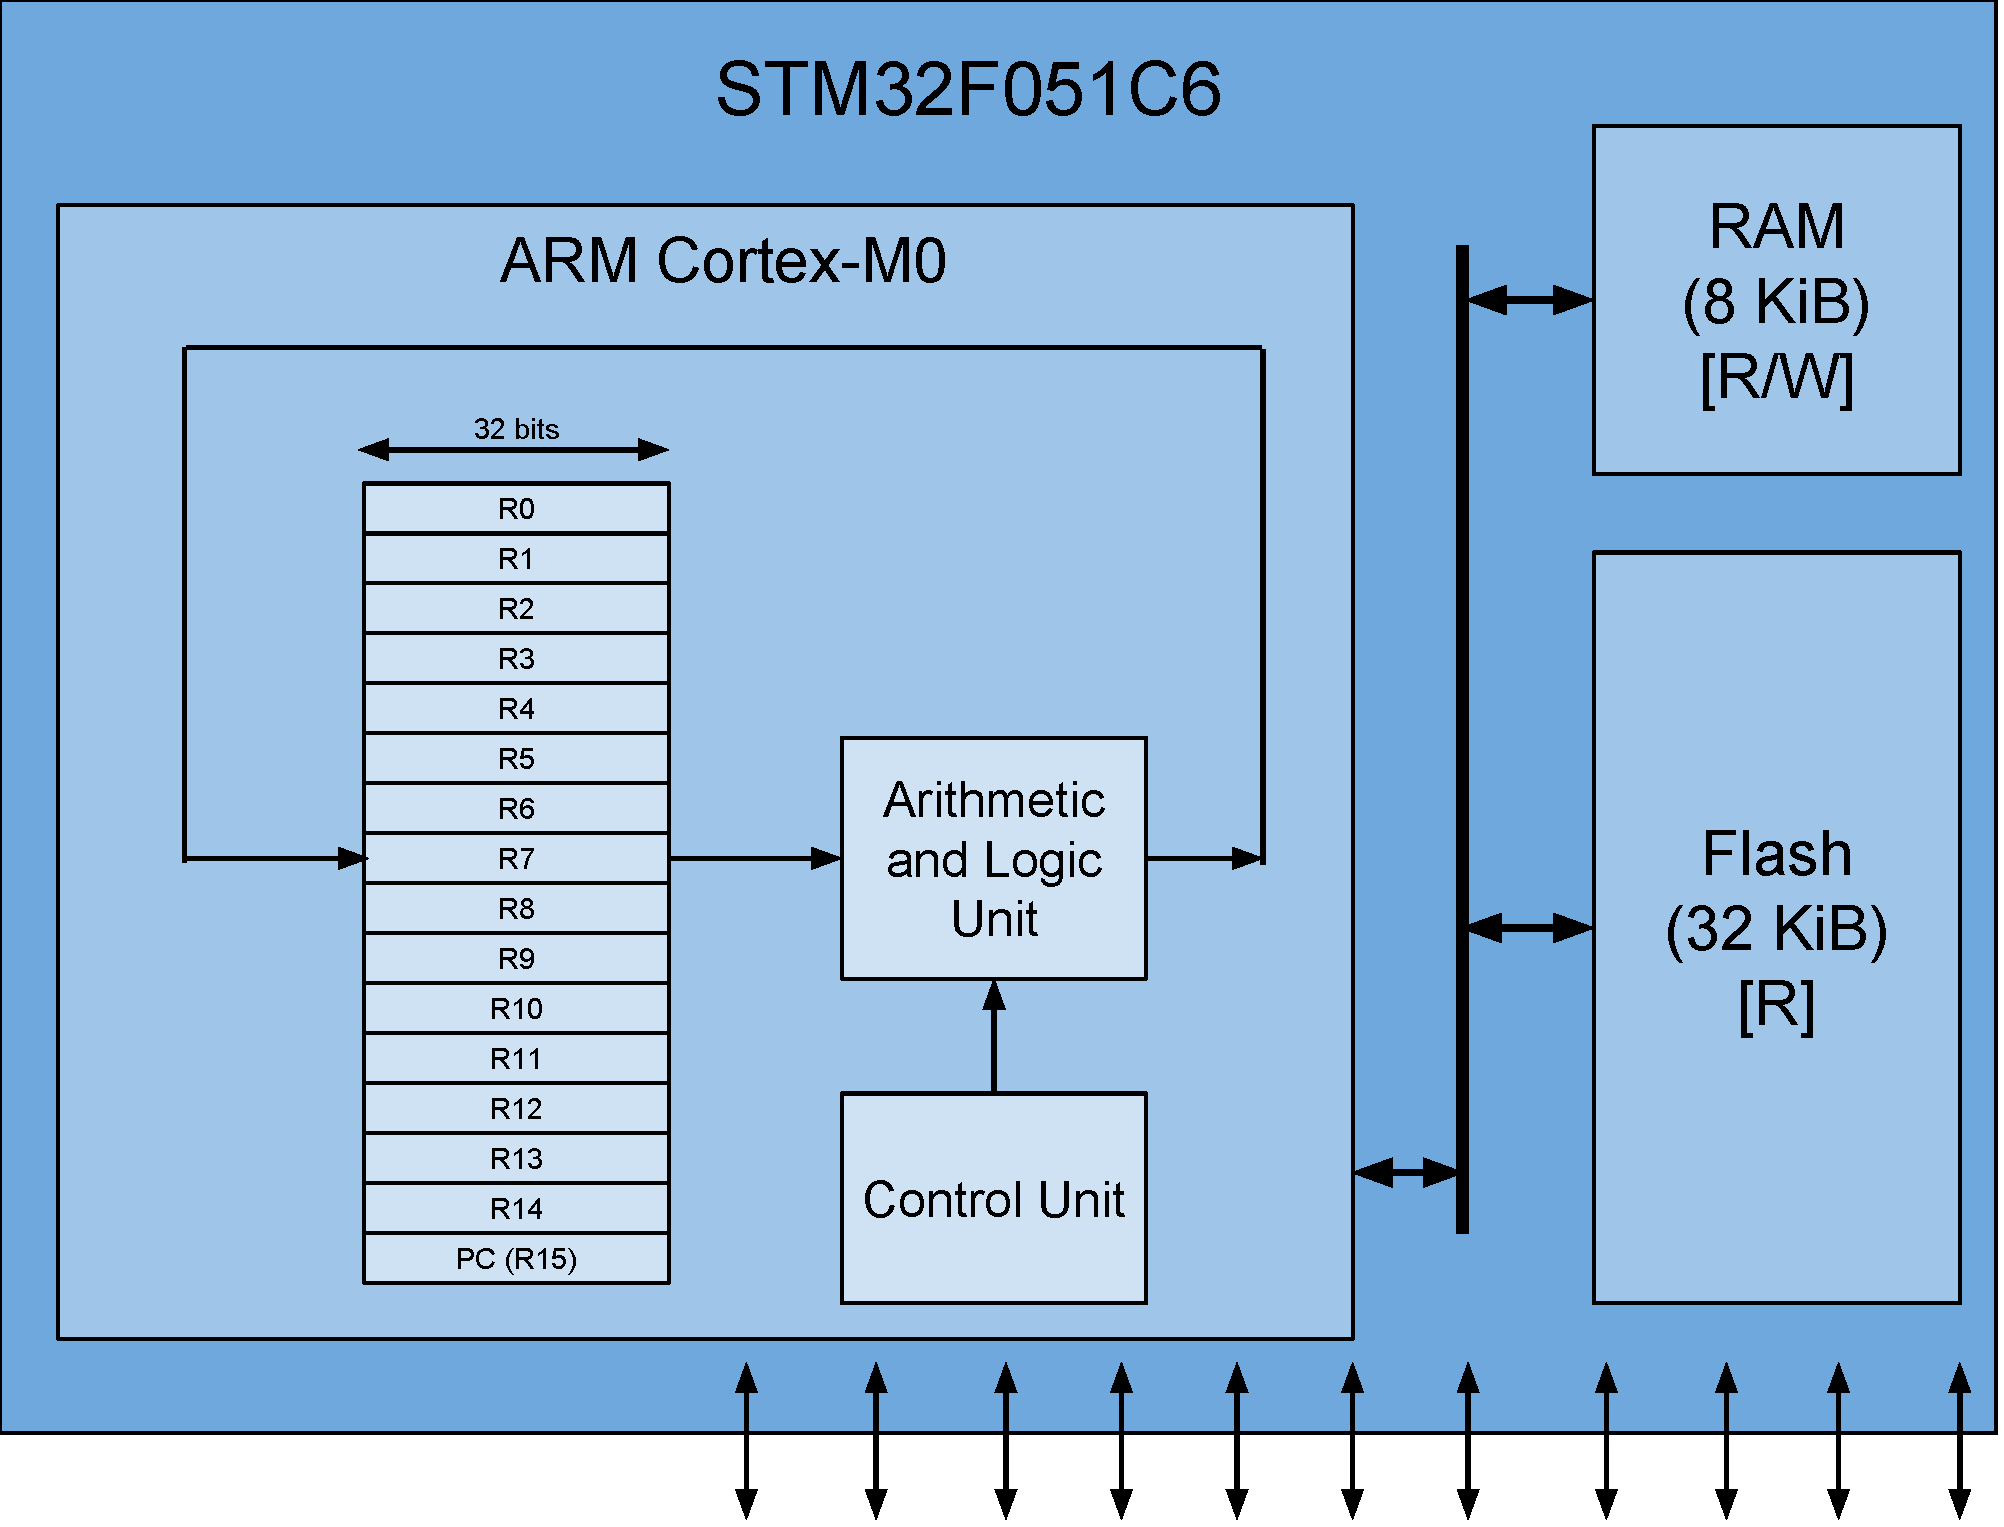
\includegraphics[width=0.9\textwidth]{./week1/programmers_model_v1.pdf}
  \caption{A view of the internals of the STM32F051 with the ARM Cortex-M0 expanded}
  \label{fig:prog_mod_v1}
\end{figure}
A programmer's model is a representation of the inner workings of the CPU with sufficient detail to allows us to develop code for the CPU, but no unnecessary detail. The expanded view of the CPU which will now be discussed can be seen in \autoref{fig:prog_mod_v1}. This simple model of a CPU is a set of CPU registers, an Arithmetic and Logic Unit (ALU) and a control Unit. The CPU registers are blocks of storage each 32 bits wide which the CPU has the ability to operate on. Only data which is inside a CPU register can be operated on by the CPU. The ARM Cortex-M0 has 16 such registers. 

The ALU is that which performs the operations on the registers. It can take data from registers as inputs, do very basic processing and store the result in CPU registers. 

The control unit manages execution by telling the ALU what to do. Together, the registers, ALU and control are able to execute instructions. 
Examples of instructions which the CPU is able to execute:
\begin{enumerate}
  \item adding the contents of R0 and R1 and storing the result in R6
  \item copying the contents of R3 into R0
  \item doing a logical XOR of the contents of R3 with the contents of R4 and storing the result in R3
  \item moving the number 42 into R5
\end{enumerate}


\section{CPU Architecture}
This section will explore some CPU architectures and compare them to the architecture of the Cortex-M0.

The Cortex-M0 makes use of a Von Neumann architecture. This means that there is a single bus which connects all of the parts (such as CPU, RAM, flash)  inside the microcontroller. The implication of this is that the CPU cannot fetch an instruction from flash at the same time as it moves data in or out of RAM. This limitation allows for a much simpler architecture, but at the expense of performance. 

Other microcontrollers (even others in the Cortex-M series like the Cortex-M3) follow a Harvard architecture, meaning that there are separate buses used for fetching instructions and moving data around. This allows faster execution as instructions can be fetched at the same time as data is loaded or stored. However, it necessitates greater complexity and more transistors. \\

It's been said that the ARM Cortex-M0 is a 32-bit processor. For comparison, the procesor which we used in this course previously (MC9S08GT16A) was an 8-bit processor. Your personal computer probably has a 64-bit CPU. 16-bit CPUs are also quite common. So what exactly does it mean when we say that the processor is 32-bits? Essentially, the number of bits which a processor is said to be referes to the size of the data bus. In other words: the amount of data which the processor is able to move around internally or perform arithmetic and logic operations on. Hence, with a 32-bit processor, we can move 32 bits of data from one spot in memory to another in just once instruction. If you had a 8-bit processor, it would cost 4 instructions to move 32 bits of data around.  

\subsection{Three stage pipeline}
Before discussing how loads or stores are done, the processor pipeline should be understood as it affects how the load instruction works. 
The ARM Cortex-M0 implements a three stage pipeline. This means that an instruction is broken up into three parts, and executed over the course of three clock cycles. The parts are:
\begin{itemize}
\item \textbf{fetch:} the instruction which the program counter points to is pulled into the CPU.
\item \textbf{decode:} the CPU control unit "looks" at the 16 bits which represent the instruction, and figures out what action it must take.
\item \textbf{execute:} the CPU runs the instruction, causing data to be modified.
\end{itemize}
The fact that the CPU is pipelined means that different instructions can be going through different phases \emph{at the same time}. In other words, one instruction can be being fetched while another is being decoded while another is being executed. 
As an example, assume we have three instructions which we want to execute, instruction A, instruction B and instruction C. The three instructions being run through the pipeline is shown graphically in \autoref{fig:pipeline}. It's critical to note how the program counter is always pointing to the instruction being \emph{fetched}. This makes sense as the job of the program counter after all is to facilitate keeping track of which instruction must be fetched. For this reason, when an instruction is being executed, the PC is actually pointing to two instructions (four bytes) further ahead in memory, and \emph{not} at the address of the instruction in execution. Hence, when an instruction in execution uses the PC, the value which will be used is the address of the instruction plus four.
\begin{figure}
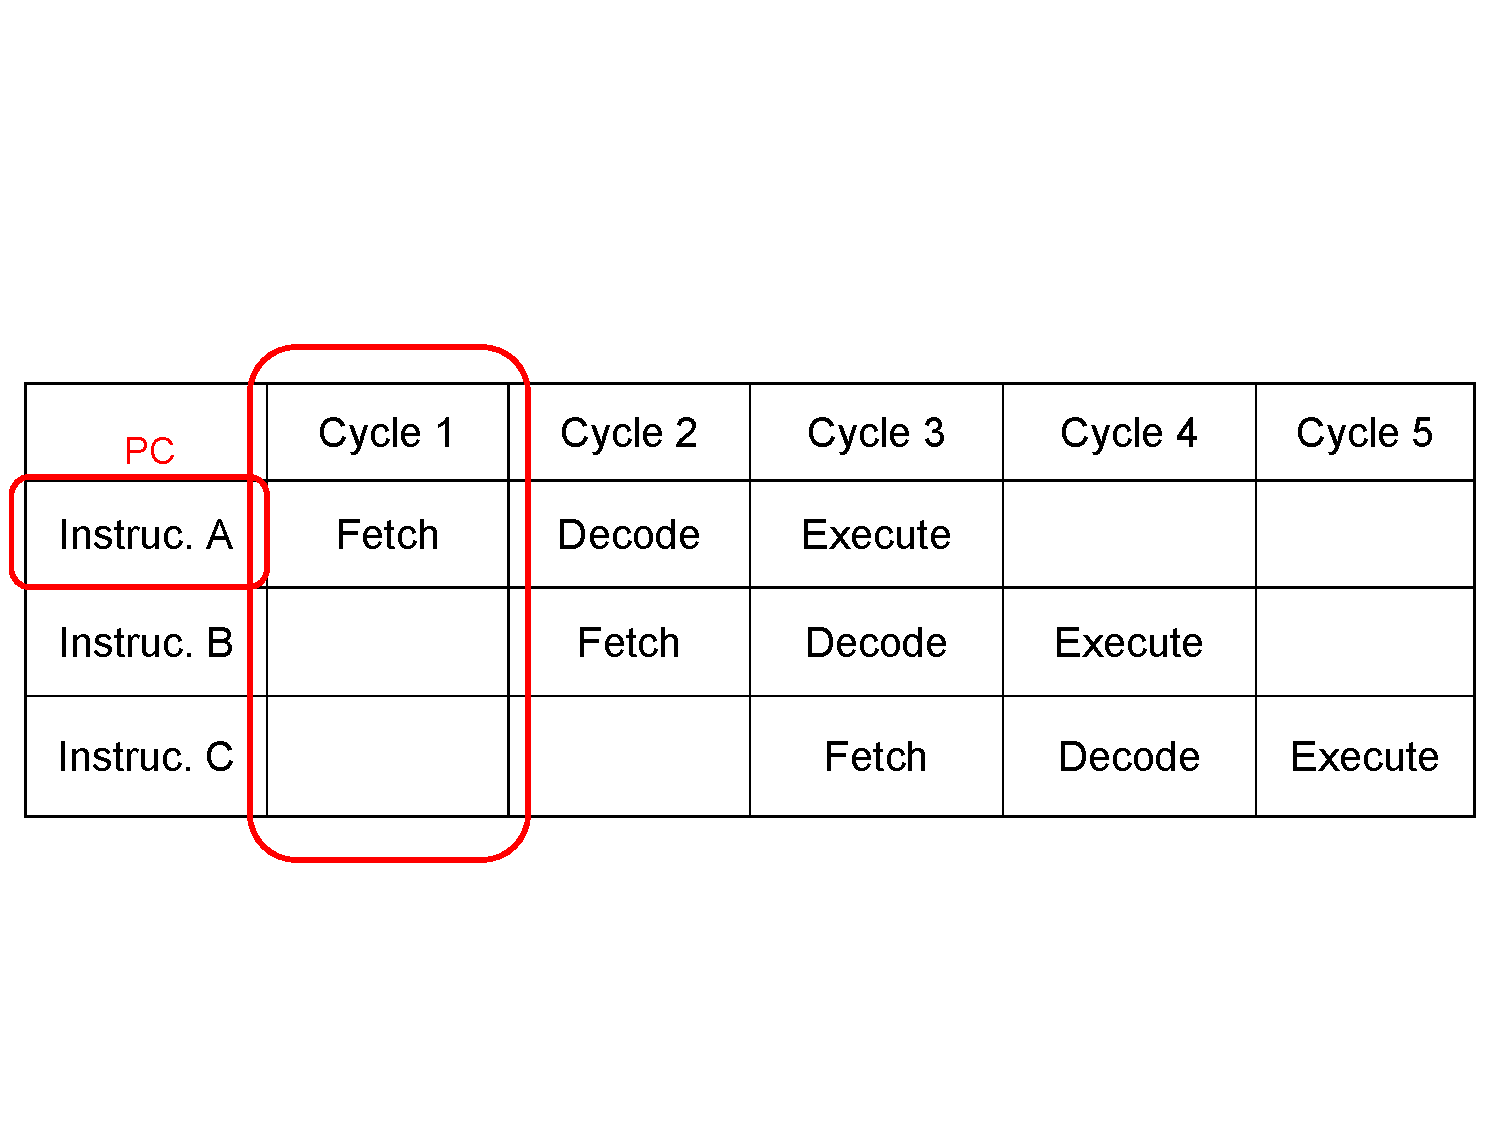
\includegraphics[page=1, clip=true, trim=1mm 40mm 1mm 57mm, width=\textwidth]{./week2/pipeline}
\includegraphics[page=2, clip=true, trim=1mm 40mm 1mm 57mm, width=\textwidth]{./week2/pipeline}
\includegraphics[page=3, clip=true, trim=1mm 40mm 1mm 57mm, width=\textwidth]{./week2/pipeline}
\caption{Showing three instructions being run through a three stage pipeline, as well as where the PC is pointing every cycle}
\label{fig:pipeline}
\end{figure}

\chapter{Coding}

\section{Assembly}

In order to get the CPU to do some of what we've discussed above, it needs to have code loaded onto it to run. We write code in a language called assembly. Assembly is a human-readable language. A program is made up of a sequence of instruction; each instruction gets executed by the CPU. It's quite easy to see what each instruction does by reading the program.  The complete instruction set is located in the Programming Manual. You must be familiar with this document! Examples of instruction which carry out the tasks listed above are:
\begin{enumerate}
  \item \texttt{ADDS R6, R0, R1}
  \item \texttt{MOV R0, R3}
  \item \texttt{EORS R3, R3, R4}
  \item \texttt{MOVS R5, \#42}
\end{enumerate}
The CPU does not have the ability to understand our nice English words like \textit{ADD} or \textit{MOV}. The CPU only has the ability to understand binary data. Assembly code must be compiled to machine code. A machine code instruction is a binary string, 16 bits long consisting of the operation code (opcode) and the data which it must operate on (operand).
For example, assume that we wanted to ascertain the machine code representation of the instruction \texttt{ADDS R6, R0, R1}. An extact from the ARMv6-M Architecture Reference Manual is shown in \autoref{fig:adds_encoding} where Rd is the destination register and Rm and Rn are the source registers of the add. It can easily be seen that the instruction would compile to\texttt{ 0001100 001 000 110 = 0x1846}.
\begin{figure}
\centering
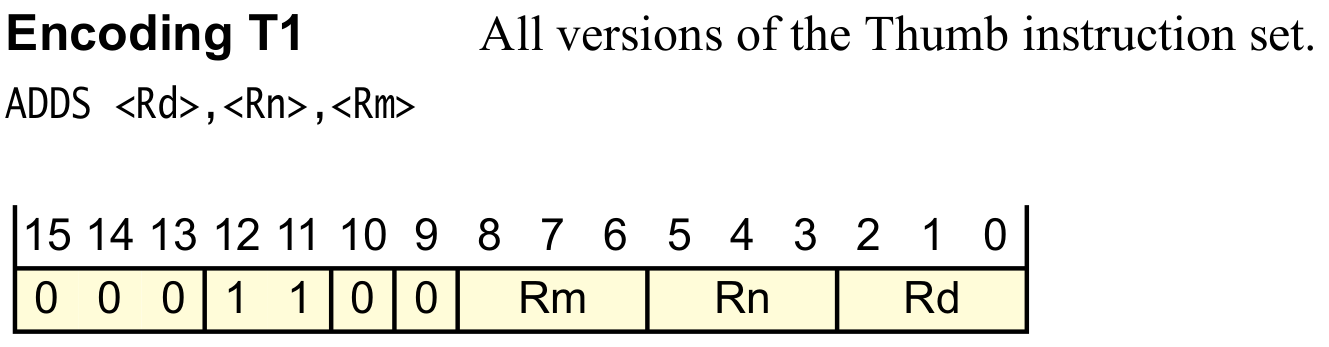
\includegraphics[width=0.7\textwidth]{./week1/adds_encoding}
\caption{An encoding of the ADDS instruction}
\label{fig:adds_encoding}
\end{figure}
The opcodes for each instruction are detailed in the ARMv6-M Architecture Reference Manual.
All of the instructions in the program are 16 bits long and are stored sequentially after one another in flash memory. 


\subsection{Instruction Sets}
An instruction set is the collection of all of the instructions which a processor can execute. 
The ARM Cortex-M0 uses the ARMv6-M architecture and this architecture supports the Thumb instruction set (as opposed to Thumb-2 or ARM). 
Thumb contains about \emph{XXX} instructions, each of which is 16 bits long. \\

Higher end ARM processors such as the Cortex-M3 or Cortex-M4 support the ARMv7-M architecture which allows multiple instruction sets to be supported by the processor. 
The ability to support multiple instruction sets requires \emph{interworking}. Interworking is the ability to specify to the CPU which instruction set to use. 
While our ARM Cortex-M0 only supports the Thumb instruction set, there is no need for interworking, yet the cabability has still been incorperated into the architecture to allow for compatability to other processors. 
This means that although our processor only supports one instruction set (Thumb), we have to explicity tell it that we are using that instruction set. 


\section{Linking}
Once our assembly code has been written and compiled to machine code, the computer which loads the code onto the micro has to be told what addresses to place the code at. The code should be placed starting at the beginning of flash.

\subsection{Executing Code}
The PC always points to the instruction which is about to be fetched. Hence, when your micro boots up, before it has executed anything, the PC will point to the first instruction to be fetched/decoded/executed.
By "point to" we mean that it holds the address of the instruction. 

As each instruction in the ARM Cortex-M0 instruction set it 16 bits (aka: half a word) long, ARM have implemented a rule that all instructions must be half word alligned. In other words, the address of the instruction must be divisible by 2 bytes. Legal addresses for instructions are hence, 0x02, 0x04, 0x06, 0x08 ... etc. 
This means that the least significant bit (bit 0) of the PC register is unused in specifcying the address of an instruction. 
Hence, it has been assigned another use. Specifically, to indicate the instruction set which is being executed. 



\chapter{Loading and Storing}

Loading is the process of getting data from somewhere in the memory space into the CPU registers so that it can be used in processing. Storing is the process of getting data which is in the CPU registers into memory. Remember that seeing as flash is read-only memory, we cannot store data to flash address, but we can store to RAM.

The general format for a load is that a destination register, a register containing a base address, and an offset are supplied. An effective address is then calculated as the base address plus the offset. The contents of memory at the effective address are then copied from memory into the destination CPU register. When we do this we are treating a register as a \emph{pointer}. When we regard the contents of a register as a memory address and use that register to access data in memory we are dereferencing a pointer: accessing the data pointed to by a pointer. This is an important concept!

A store operation is very similar. Again, a register containing a base address and an offset are supplied, but this time it is a source register not a destination register which is supplied. Again, and effective address of base plus offset is calculated. The contents of the source register is copied into the effective address. 

Note that most of the load/store operations which we will be doing are 32-bit (word) load or stores. This is because the CPU registers are 32 bits. So far we have only spoken of a single effective address. As you know, each address can only hold 8 bits. Hence, in order to load or store 32 bits, four sequential addresses are used. The effective address specifies the \emph{lowest} in the sequence of the addresses. For example, if we wanted to store the contents of R0 in 0x20000000, the word would be placed into the address range 0x20000000, 0x200000001, 0x20000002 and 0x20000003. Remember that our processor uses little endian format, so the LSB is placed at 0x20000000 and the MSB at 0x20000003.

We will now explore some implementations of loading and storing.

\section{Immediate Offset Loading}
In this format, the base address is supplied in one of high CPU registers (R0 - R7), and the offset is supplied as an immediate number. 
The instruction format for loading data into a register is
\begin{lstlisting}[fontadjust=true,frame=trBL]
LDR Rt, [Rn, #imm]
\end{lstlisting}
where \texttt{Rt} is the target register for the load, \texttt{Rn} contains the base address and \texttt{\#imm} is the offset from the base address.

The way that this instruction works is that it calculates an \emph{effective address} which is equal to the contents of the base address register plus whatever number is supplied as an immediate operand.
There is, however, a slight complexity in how the offset is dealt with.

\subsection{Offset restrictions}
\label{sec:load-store-restrictions}
Remember that all instructions are limited to 16 bits. The format of the LDR instruction in machine code is shown in \autoref{fig:ldr}. We can see that after 5 bits of opcode and $2 \times 3 = 6$ bits of register specifications, we are only left with 5 bits of offset. Normally, these 5 bits would only allow us to provide an offset of $2^5 - 1 = 31$ bytes. This is not very much! In order to extend the range of the 5 offset bits, the actual offset used is equal to the 5 bit immediate number multiplied by four. This multiplication by four is the same as appending two zeros to the end of the binary value, which you can see is being done in \autoref{fig:ldr}. This means that the amount which we are able to offset a base address by is now $(2^5 - 1) \times 4 = 124$, which is significantly more useful. However, seeing as we are multiplying to immediate number by four to get the actual offset, the implication is that all offsets \emph{must} be a multiple of four. 
The compiler automatically takes care of dividing whatever offset we supply in our assembly instruction by four in order to get it to fit into the 5 bit immediate number, and the CPU then multiplies the immediate number by four to get the offset.

For example: if we wanted an offset of 12, the immediate number which would be placed in the instruction by the compiler would be 3.

\begin{figure}
\centering
\includegraphics[page=139, clip=true, trim=35mm 157mm 55mm 40mm, width=0.85\textwidth]{./DDI0419C_arm_architecture_v6m_reference_manual}
\caption{Machine Code representation of LDR instruction. Source: ARMv6-M Architecture Reference Manual}
\label{fig:ldr}
\end{figure}

\section{Program Counter Relative Loading}
There is another format of the LDR instruction which takes the Program Counter as a base register, and allows for an 8-bit immediate offset. If you wish to load data from flash into a CPU register, it makes sense to use the PC as a base register due to the fact that the PC is already initialised to be pointing to an address in flash. Specifically, it is pointing to the instruction which is being fetched (not executed - remember the three stage pipeline!). The format of the LDR instruction for PC relative loading can either be specified in the same was as the general LDR instruction, or it can have a label provided as an operand, as follows:
\begin{lstlisting}[fontadjust=true,frame=trBL]
LDR Rt, [PC, #imm]
LDR Rt, <label>
\end{lstlisting}
If one supplies a label as an operand, all that the compiler does is calculate the correct immediate offset value to insert, and compiles the instruction as if it were in the first format. It's important to note that these instructions are exactly equivalent: all that using a label does is cause the compiler to do the hard work of calculating the correct offset so you don't have to. It would really be a lot of hard work; every time you changed something in the structure of your program which caused instructions to be moved to different memory addresses (like writing a new line of code!) you'd potentially have to re-calculate your offsets. The ability to use labels is one of the most useful features of the compiler.


\section{Register Offset Loading}
So far all offsets have been supplied as immediate numbers to the load instructions. However, there is another format of the load instruction called a register-offset load. Here, the offset is contained in another register. This is useful as the offset can be set at run-time by modifying the contents of a register, rather than at compile time. In this case, the effective address is calculated as the contents of the base register (\texttt{Rn}) plus the contents of the offset register (\texttt{Rm}). 
\begin{lstlisting}[fontadjust=true,frame=trBL]
LDR Rt, [Rn, Rm]
\end{lstlisting}

\section{Storing}
The storing commands are so similar to the loading that they will barely be discussed. One difference is that there is no PC-relative store, as there would be no point trying to store data to read-only memory. The store instruction takes moves the contents of a source register, \texttt{Rt}, and places it at the effective memory address equal to the base address, \texttt{Rn}, plus an offset either supplied as a 5-bit immediate number, \texttt{\#imm5}, or in an offset register, \texttt{Rm}.

\begin{lstlisting}[fontadjust=true,frame=trBL]
STR Rt, [Rn, #imm5]
STR Rt, [Rn, Rm]
\end{lstlisting}

\section{Accessing of Datatypes Other Than Words}
So far we have only loaded or stored words. While it is useful to be able to move an entire 32 bits of data around at once we will sometimes only want to move bytes of half-words around. There are instructions which allow us to do this. There is a version of the \texttt{LDR} instruction which loads only 1 byte: \texttt{LDRB}. Similarly, there is a version which loads 2 bytes or half a word: \texttt{LDRH}. 

\chapter{Branching}
Branching refers to the ability to alter the order of execution of code. Ordinarily the instructions which are coded and then placed into flash are executed sequentially: one after the other in the order which they appear in flash. However, this is highly limiting. Branching allows us to execute instructions which can cause the CPU to jump to executing any instruction in the program (sort of). 

\section{Implementation of a Branch}
Seeing as the program counter (PC) entirely specifies which instruction is going to be executed next (by holding the address of the instruction) it is relatively simple in concept to get the CPU to execute a specific instruction: write the address of that instruction to the PC. Unfortunately there is a complication.

Due to our instructions being 16 bits wide, it is not possible to hold the address of an instruction to branch to as immediate data seeing due to addresses being 32 bits (you can't fit 32 bits of operand into a 16 bit instruction!).
To overcome this, a technique called relative branching is employed. This means that the address of the instruction which the CPU branches to is equal to the contents of a certain register plus or minus a certain amount. Seeing as the PC is already pointing to the general area in memory where instructions live, the PC is most often use as the base address register. This means that the branch instruction causes the PC to take on a value equal to the current value of the PC plus/minus some amount. 

\section{Using labels}
We could manually calculate the difference between the addresses of instructions which we wanted to branch to/from and use that as our offset address. However, just as in the case of load/store, this would be exceptionally tedious. We can use labels to get the compiler to do the laborious work calculating offsets for us. Similar to load/store instructions, we can label an instruction and then use that label as a operand for a branch instruction. The compiler then works out the address of the instruction which has been labeled, works out the address of the instruction which is doing the branch and creates a PC relative branch instruction with the correct offset equal to the difference in addresses of the two instructions. 

For example, consider something like this:
\begin{lstlisting}[fontadjust=true,frame=trBL]
foo: LDR R0, [R1]
 ADDS R0, R0, #1
 ...
 ....   @ a whole lot of other instructions
 B foo
\end{lstlisting}
That would work by calculating the difference between the branch instruction and the instruction labeled \texttt{foo} and then subtract that amount from the PC when the branch took place. There are slight complications around things like the three stage pipeline and data alignment optimisations but in principle that's how it works. 

\chapter{Perihperals}
%Ports are typically controlled by a block of memory called perihperals. Unlike RAM which is general purpose, each register in the perihperals memory block has a specific, well defined purpose. Typically the purpose of these perihperal registes are for configuring the microcontroller to behave in a certain way or communicate with the outside world.
%These CPU registers are different to the peripheral registers mentioned earlier for the reasons that they are located inside the CPU rather than in the address space and also they are mostly general purpose: they can hold any data required in the execution of a program. 

\chapter{Clock Distribution}
In order for a block of circuitry to function inside the microcontroller it needs to be clocked. Clocking circuitry provides it with well defined timing which allows the circuitry to take data from the bus or place data onto the bus exactly in sync with all other circuitry in the microcontroller. This essentially enables the circuitry for use. However, as soon as circuitry inside the micro is clocked/enabled, it draws power. For that reason, each internal peripheral can selectively be enabled or disabled by providing or removing (better known as \emph{gating}) the clock to that peripheral. Most importantly the clock is default \emph{OFF} for all peripherals in order to make the default power consumption as low as possible. The exact amount of power consumed by each peripheral is different depending on which peripheral it is. Furthermore, power consumption is approximately linear with clock speed. At maximum clock speed the power consumption is roughly half a milliamp per peripheral. 

\section{Reset and Clock Control}
The RCC is a peripheral. As the name implies, one of its key functions in the management of the clocking system of the microcontroller. This involves both generating or altering the clock frequency and selectively gating or allowing clock to the other peripherals of the micro. 

The peripherals are divided up into a bus structure as shown earlier and as such the structure of the clock distribution is also based on a bus structure. The RCC has a register for each bus. The register controls the state of the clock of the devices connected to that bus. These registers include the RCC\_AHBENR, RCC\_APB1ENR and RCC\_APB2ENR. 

\subsection{Clock Source}
As well as managing the gating of clocks for peripherals the RCC also selects the oscillator which should be the source of the system clock (sysclock). The default source is an internal 8 MHz RC oscillator. Optionally, the external crystal quartz oscillator can be selected as clock source. The advantage of using an internal oscillator is that it does not require an extra component to be connected to the micro. The disadvantage is the tolerance: it is around 1\% at room temperature, but can be more than 4\% at more extreme temperatures. The tolerance of an external crystal quartz oscillator is typically much better than 0.01\%. Hence, for applications which are not timing sensitive the internal oscillator can be used. For timing sensitive applications the external oscillator should be used. 

\section{CPU Instruction Cycles}
As well as driving the peripherals the system clock drives the CPU. The instructions which we write each take a certain number of CPU cycles to execute. Instructions typically take one cycle to execute, but this is not true for all instructions. The exact number of cycles which can instruction takes is detailed in Section 3.3 of the ARM Cortex-M0 Technical Reference Manual. By knowing how many cycles each instruction takes to execute we can know how many cycles a specific block of code takes to execute. By knowing how long each cycles takes in real time (this is the inverse of frequency) we know the real time which a block of code takes to execute. 

\chapter{General Purpose Input/Outputs}

\chapter{Conditional Branching}
The branching we have done up until now has been unconditional branching: the branch instruction is always executed. This is highly limiting as the program can have only one flow. Conditional branching refers to the ability of the CPU to either take or ignore a branch instruction depending on some condition. This is very powerful as it allows the flow of the program to by variable depending on dynamic conditions. 

\section{Application Program Status Register}
The APSR is a special CPU register. It does not have a register number like the other registers and cannot be read or written by normal instructions. However this is a critically important register as it is the source of the conditions for the conditional branching. The APSR holds 4 flags:
\begin{description}
\item[Negative (N):] Set if the result of the last operations has was negative. In other words, the msb was a 1. This flag only has a meaning when treating data as signed numbers. 
\item[Zero (Z):] Set if all bits of the last operations were 0.
\item[Carry/Borrow (C):] Set if an \emph{unsigned} overflow occurred. Ie: the actual result of the computation exceeded the bounds of the 32-bit register when treated as an unsigned number.
\item[Two's Compliment Overflow (V):] Set if a \emph{signed} overflow occurred. Ie: the actual result of the computation exceeded the bounds of the 32-bit register when treated as a signed number. 
\end{description}

Together, these flags provide us with an abundance of information about the result of computations. We are able to ascertain basically any information about the relationship between arbitrary numbers by examining these flags. Not all instructions set the APSR flags. It is necessary to examine the details of the instruction in the Programming Manual in order to see whether the instruction sets the flags. Furthermore it may be necessary to examine the detailed workings of the instruction in the ARMv6-M Reference Manual in order to see which flags are set and how the settings of those flags is determined. However, in general instructions which set the flags have an \texttt{S} at the end of their name. Again (in general) arithmetic operations set/clear all APSR flags while logic operations set/clear only the \texttt{N} or \texttt{Z} flags. 

\section{Compare Instruction}
One of the key instructions used in the context of conditional branching is the compare (\texttt{CMP}) instruction. This instruction essentially subtracts two values from each other, disregards the result but updates the flags depending on the result. \texttt{CMP} takes either two registers or a register and an immediate value as operands. The CMP instruction is most often used to set the conditions which the conditional branch will depend on. This is due to the fact that a subtraction tells us a lot about the relationship between two numbers. For example, if the result of a subtraction sets the zero flag we know that the numbers being compared (subtracted) have the same value. Similarly, if the result of the subtraction of B from A clears the V flag it tell us that A is larger than B when viewed as signed numbers. 

The format of the \texttt{CMP} instruction is one of:
\begin{lstlisting}[fontadjust=true,frame=trBL]
CMP Rn, Rm
CMP Rn, #imm8
\end{lstlisting}
In the first case, the value of Rm is subtracted from Rn. In the seconds case, the 8-bit immediate number is subtracted from Rn.

\subsection{A note on the implementation of the subtract operation}
In order to minimize the hardware cost of the ALU circuitry, the subtract operations is implemented by adding the bitwise inverse of Rm to Rn, plus 1. You don't really have to worry about this other than to note that this implementation explains why the C or V flag is set when the numbers being compared are equal. For example, the subtraction of the number 42 from the number 42 corresponds to the addition of the numbers 42 and 4294967253 and 1. It should be apparent to you that this result is zero, but sets the carry flag. 


\section{Condition Code Suffixes} 
The branch (\texttt{B}) instruction is able to take optional condition code suffixes which specify whether or not the instruction will be executed depending on the state of the flags in the APRS. 
These suffixes are shown in \autoref{fig:cc_suff}. A suffix can be appended to the \texttt{B} instruction to turn it into a conditional branch. For example, \texttt{BEQ} will be taken if the result of the last computation produced a zero result. Similarly, \texttt{BNE} will be taken if the result was non-zero. 

The mnemonics for the suffixes are closely related to the compare operation. For example, the BGT (branch if greater than when treated as signed numbers) will be taken if the Rm operand of the CMP instruction is greater than the Rn operand when treated as signed numbers. This is why the CMP and B\{cc\}  instructions go so well together.

\begin{figure}
\centering
\includegraphics[page=40, clip=true, trim=110 130 60 434, width=\textwidth]{./stm32f0xx_programming_manual}
% left, bottom, right, top
\caption{Condition code suffixes and meanings. Source: Table 17, Programming Manual}
\label{fig:cc_suff}
\end{figure}

\section{Branching Based on Individual Bits}
Consider the case where we want to take a branch conditional on the case of a push button being pressed or not pressed. A push button is connected to a single pin which constitutes a single bit in the GPIO\_IDR. Hence, we need a way to make our branch conditional on a single bit being high or low. Put another way, we want to exclude all of the other bits in the IDR from influencing the branch. 

In order to achieve this we have to do two steps:
\begin{enumerate}
\item Mask out the bits which we are not interested in. Specifically, set them all to zero. This is done just as we saw earlier in \autoref{sec:set_clear_individual_bits}. We AND all of the bits with 0 except for the bit which we are interested in which we AND with 1.
\item Compare the result of the mask with 0. If the bit which we are interested in was 0 then the result of the AND will be 0. If the bit that we are interested in was 1 then the result of the AND will be non-zero. Note that this compare does not actually have to be done as the AND instruction sets or clears the zero flag.
\end{enumerate}
After those two steps (which can actually just be one step) we can take a conditional branch dependant on whether a single bit (a single push button) was set or cleared. 

\chapter{Instruction Sets}
An instruction set refers to a collection of instructions which a CPU is able to execute. This is a combination of the assembly instruction names and the machine code which the assembly language is compiled down to and which is placed into memory for execution. There are three different instruction sets which various ARM processors use. These are Thumb, Thumb-2 and ARM. A graphical representation of the instructions which are available on the various Cortex processors is shown in \autoref{fig:isa}. Here we see that the Cortex-M0 and -M1 use the Thumb instruction set while the -M3 and -M4 use the Thumb-2 instruction set. Following is a short discussion on each of the three instruction set which ARM supports. Note while reading that our processor (the Cortex-M0) only supports Thumb instructions\footnote{Not quite true. It supports 3 Thumb-2 instructions. Why 3? I don't know...}.

\begin{figure}
\centering
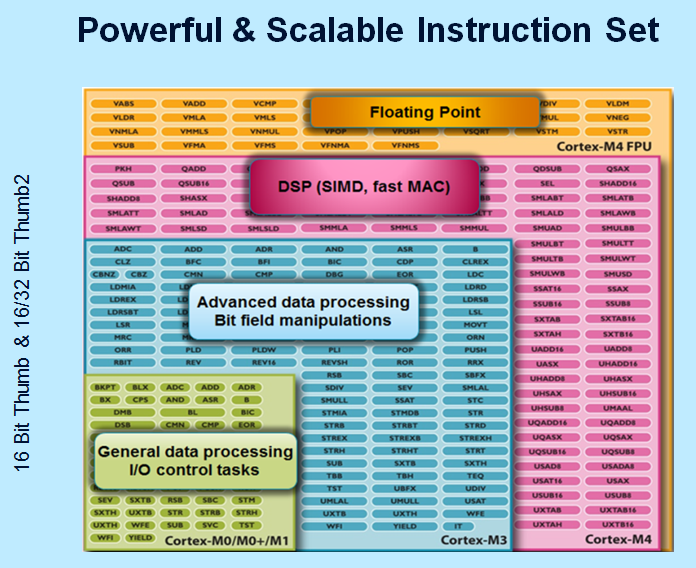
\includegraphics[width=\textwidth]{./week5/ISA}
\caption{Cortex instruction set architecture}
\label{fig:isa}
\end{figure}

\section{ARM}
The original instruction set used by ARM processors was called the ARM instruction set. This instruction set contains only 32-bit instructions. This is a powerful instruction set as almost all instruction can be conditionally executed. However, seeing as all instructions are fixed to 32 bits wide, the code density is fairly poor. This is due to comparatively simple instructions like a simple add or PC relative branch using wasteful 32 bits of flash.

\section{Thumb}
In 1994 the ARM7TDMI architecture was released which featured the Thumb instruction set. This instruction set was limited to only 16-bit instructions. Obviously these instructions were less powerful as there was less room to specify information about the actions which an instruction should perform. However for simple instructions this was not an issue and resulted in programs being much smaller. For more complicated operations multiple Thumb instructions would be needed to perform the job of a single ARM instruction. 

In order to have a combination of the performance of the 32-bit ARM instruction set and the code density of the 16-bit Thumb instruction set, an ability called \emph{interworking} was provided. Interworking allows for the CPU to switch between executing Thumb instructions or ARM instructions. This is a useful ability but introduces some additional complexity into the system.

\section{Thumb-2}
Thumb was extended to Thumb-2 in 2003. Thumb-2 allows 16-bit and 32-bit instructions to be freely mixed together without requiring interworking. Essentially Thumb-2 is a combination of the 16-bit instructions provided in Thumb as well as a whole lot of extra 32-bit instructions. This instruction set allows performance similar to the ARM instruction set while providing code density even better than Thumb. 

It's important to note the structuring of the instruction sets: As shown in \autoref{fig:isa}, Thumb-2 (Cortex-M3 and -M4) entirely contains all of the 16-bit instructions of Thumb (Cortex-M0 and -M1). Any Thumb code will run on a Thumb-2 capable processor. Any Thumb-2 code will probably NOT run on a Thumb processor. This is called backward compatibility (sort of). The ARM instruction set is completely distinct from that figure. It is a completely different instruction set which does not run on the Cortex series of processors. Processor architectures which support Thumb and ARM (such as the ARM7TDMI) require interworking to switch between the two entirely distinct instruction sets.

\section{Implementation of Interworking}
So we understand that Thumb processors can only execute 16-bit instructions. Thumb-2 processors can execute the Thumb instructions as well 32-bit instructions. ARM processors can execute a totally different set of 32-bit instructions. Some processors can run both the ARM and Thumb instruction sets. So, how do we tell one of these interworking capable processors whether an instruction is ARM or Thumb?

Firstly, note that data accesses must be aligned. Seeing as the minimum width of an instruction is 2 bytes, all instructions must be placed on  addresses which are multiples of 2. As all addresses of instructions are multiples of 2, the lsb of the PC is always a 0. The bit is therefor sort of wasted. Hence, we assign a different purpose to this bit: when it is a 0 it indicates that the instruction pointed to by the PC is an ARM instruction. When it is a 1 it indicates that the instruction pointed to by the PC is a Thumb instruction. 

Although the Cortex series of CPUs does not support the ARM instruction set, is still requires that this rule of using the lsb of the PC to specify instruction set type is adhered to. Seeing as all instructions for the Cortex series (including our CPU) are Thumb or Thumb-2, this lsb of the PC should always be set to a 1. That is why our reset vector needs to point to the address of \texttt{\_start} +1. The +1 forces the lsb to a 1 indicating that the instruction at \texttt{\_start} is a Thumb instruction. 

If a vector attempts to set the lsb of the PC to 0, the CPU will HardFault as it would be trying to execute an instruction from an instruction set which is not supported. 

\chapter{Exceptions}
\label{sec:exceptions}
An exception is a fairly generic term for an event which occurs which the CPU needs to deal with in some way. Examples of exceptions would be the microcontroller resetting or the CPU attempting to access invalid memory or a peripheral generating an interrupt. Typically we write a block of instruction which we want to execute when an exception occurs. That block of code is called an \emph{exception handler}. We then place the address of the start of that exception handler into a special location in memory called a vector. Each exception has a vector address associated with it. The block of all vectors is called the vector table. A summarised version of it is shown in \autoref{fig:vector_table_summarised}.

\begin{figure}
\centering
\includegraphics[page=23, clip=true, trim=60 476 68 168, width=\textwidth]{./stm32f0xx_programming_manual}
% left, bottom, right, top
\caption{Summarised version of the vector table showing the CPU exceptions only. Source: Table 12, Programming Manual}
\label{fig:vector_table_summarised}
\end{figure}

When an exception occurs, the CPU performs a few tasks in order to service the exception:
\begin{itemize}
    \item Save the current 'system state' to the stack in the form of a stack frame. This is basically just pushing a few important registers to the stack. The exact format of the stack frame is shown in \autoref{fig:stack_frame}.
    \item Fetch the data from the vector associated with that exception that occurred and load that data into the PC.
    \item Start executing the block of instructions pointed to by the vector
\end{itemize}

Following is a discussion on some of the key exceptions.

\begin{figure}
\centering
\includegraphics[page=26, clip=true, trim=135 315 100 410, width=\textwidth]{./stm32f0xx_programming_manual}
% left, bottom, right, top
\caption{Stack frame. These registers are push to the stack thereby saving their state when an exception occurs. Source: Figure 9, Programming Manual}
\label{fig:stack_frame}
\end{figure}

\section{Reset}
There are a number of possible causes of a reset all detailed in section 7.1.2 of the Reference Manual. They key ones are a power reset where the power to the micro is cycles or a NRST pin reset where the Negative ReSeT pin is pulled low and then released. 

When this exception occurs the microcontroller:
\begin{itemize}
    \item aborts execution of code, 
    \item sets all registers to their default values,
    \item fetches the data from the reset vector,
    \item places that data into the PC and starts execution. 
\end{itemize}

The reset exception is fairly specialised in that is the only exception which does not cause the previous system state to be stacked. Quite the opposite in fact, it clears all state and begins fresh. 

\section{HardFault}
A HardFault occurs when an instruction attempts to do something illegal or a peripheral attempts to do an illegal memory transfer. This includes attempting to access unimplemented memory addresses or trying to perform unaligned memory access or trying to execute an instruction which has a non-existent opcode. The full list of events which cause a HardFault exception are detailed in Table B1-6 of the ARMv6-M Architecture Reference Manual.

Typically HardFaults are unrecoverable: when a HardFault happens there is generally something broken in the code and we do not want the code to carry on running. Rather we want to be made aware of the issue so that the code can be corrected. 

When a HardFault happens the standard exception handling procedure takes place: the current state is stacked, the exception handler vector is fetched an executed. Due to the fact that the state is saved on the stack it is possible to return from the handler and resume execution of the main code but it would be unusual to want to do this due to the severity of a HardFault.


%\begin{overpic}[grid,page=23]{./stm32f0xx_programming_manual}
%\end{overpic}

\chapter{Stack}
A stack is a concept. The concept is a data structure which implements a Last In / First Out queue. It has two interfaces namely:
\begin{description}
    \item[PUSH:] Take a value and places it at the top of the stack, on top of whatever already exists in the stack.
    \item[POP:] Removes the top element from the stack and puts it into a register. The next element down then becomes the top of the stack.
\end{description}

That's basically all there is to a stack: a LIFO queue. An animation of this queue in operations is shown at \url{http://www.csanimated.com/animation.php?t=Stack}

The stack is such a useful thing for computer systems what we dedicate specific hardware in the CPU to implementing one of these LIFO queues. The stack has two main uses:
\begin{enumerate}
    \item Saving system state. When an exception occurs we want to back up the system state somewhere and then have the ability to recover the backed up state later if we return from the exception. The stack provides us an always-accessible place in memory where this information can be placed and recovered later.
    \item General data storage. We have a limited number of registers yet frequently need to work with more data than our CPU can hold. While we could just pick addresses in RAM for use as data storage, we'd have to keep a list of what locations are used for what in our different blocks of code, hard code the addresses into the program and make sure that we don't overwrite our data in RAM. With a stack we can simply push data to the stack and pop it later when we want to get it back. The stack implementation keeps track of the actual memory addresses which data goes to. 
\end{enumerate}

\section{Stack Pointer}
Clearly a well implemented stack is highly beneficial to a system. In order to implement the stack, one of our registers, R13 is assigned the special job of being the stack pointer (SP). The purpose of the stack pointer is to point to (hold the address of) the item most recently placed on the stack. In that way it keeps track of the stack. Typically a stack is implemented starting at the end of RAM (highest address) and working it's way down RAM. Hence, the SP should be initialised pointing to the end of RAM.

Well, that's not quite true! As discussed in section 2.1.2 of the Programming Manual, the order of operations for a stack push is to first decrement the pointer and then place the data at the new address pointed to by the SP. That means that if we want to place our first word pushed onto the stack, the SP must be initialised to point to one word AFTER the end of RAM.

The reason we want to start the stack right at the end of RAM is to allow it as much space as possible to grow. Typically computer systems have another data structure called a heap with starts at the beginning of RAM and grows upwards. These data structures should be as far away from each other as possible to prevent stack overflow, when the stack and the heap collide. Stack/Heap collision is about the worst think that can happen to a program. This is why lots of RAM is good: the more RAM we have the more data we can store before collision happens. 

\section{Stack Access Instructions}
The two instructions which give direct access to the top of the stack are the PUSH and POP instructions. Both of these instructions take something called a register list as an argument. This is sort of an array of registers, enclosed in curly brackets such as \{R0, R2, R5\}. This is very powerful as it allows us to push or pop multiple registers at one!

Seeing as the SP is a CPU register like any other, you can also use it for load/store operations enabling the random access of any element on the stack. For example, to load the \nth{5} last element on the stack by 42 without touching any of the other elements you could do:
\begin{lstlisting}[fontadjust=true,frame=trBL]
LDR R0, [SP, #16]
ADDS R0, R0, #42
STR R0, [SP, #16]
\end{lstlisting}
Without this ability you'd have to pop off all 5 values into registers, add 42 to the specific register and then push the results back.

\chapter{Subroutines}
It would be very useful to have the ability to branch to a label, execute a block of code and then return back to where the branch was taken from. A block of code which is branched to and returned from in this way is called a subroutine.
Subroutines are a very useful concept as they allow us to write a single block of code and then re-use it multiple times. 
If we did not have subroutines we would have to duplicate code whenever we wanted to make use of the functionality provided by the code.
This causes unnecessary use (wasting) of flash memory.
Furthermore, without subroutines, the job of maintaining the code would be very difficult because if you want to adjust something in that block of code then you would have to make the adjustments in multiple places in your source file - wherever the block of code exists.
By having a subroutines the code only occupies space in memory once and alterations to it only have to happen in one place.

In order to implement this subroutine concept the CPU needs the ability to store the return address somewhere when a subroutine is branched to. 
Subroutines are so useful that an entire CPU register is dedicated to the purpose of storing return addresses for subroutines. That is R14, otherwise known as the Link Register (LR).
Subroutines work by storing the address of the next instruction to be executed in the LR and then branching to the label of the subroutine.
As you'll remember, this is the same as putting the address of the instruction which you want to execute into the PC. As usual, instruction will then be executed sequentially from that point.

In order to get the branch instruction to store the address of the next instruction in the LR, the following instruction format is used.
\begin{lstlisting}[fontadjust=true,frame=trBL]
BL label

\end{lstlisting}

When you want to "return" from the subroutine back to the location in the code where the subroutine was called you need move the data in the LR into the PC. This causes the PC to go back to pointing to the instruction which follows the one that called the subroutine. 

In order to load the contents of an arbitrary register into the PC, the Branch Indirect (BX) instruction is used.
The general format of this instruction is:
\begin{lstlisting}[fontadjust=true,frame=trBL]
BX Rn  @ where Rn is some register
\end{lstlisting}

To return from a subroutine we want to move the contents of the LR into the PC. Hence the specific format of the instruction to use is one of the following (they are equivalent) 
\begin{lstlisting}[fontadjust=true,frame=trBL]
BX LR
BX R14
\end{lstlisting}


\end{document}
